\section{Proposed approach}
\label{sec:apprach}

Our objective is to extract a catalog of reusable language modules from a given set of DSLs (that we refer to as the \textit{input set}). To this end, we propose an approach based on the aforementioned notions of overlapping and potential reuse. Concretely, in our approach we first identify syntactic and semantic overlapping among the DSLs of the input set. Then, we cut such overlapping in order to break-down the DSLs in reusable language modules. Those language modules are encapsulated in such a way that they can be later composed among them to obtain complete DSLs. The overall strategy is illustrated in Figure \ref{fig:breakingdown}. This section is dedicated to explain it in detail.

\begin{figure}
\centering
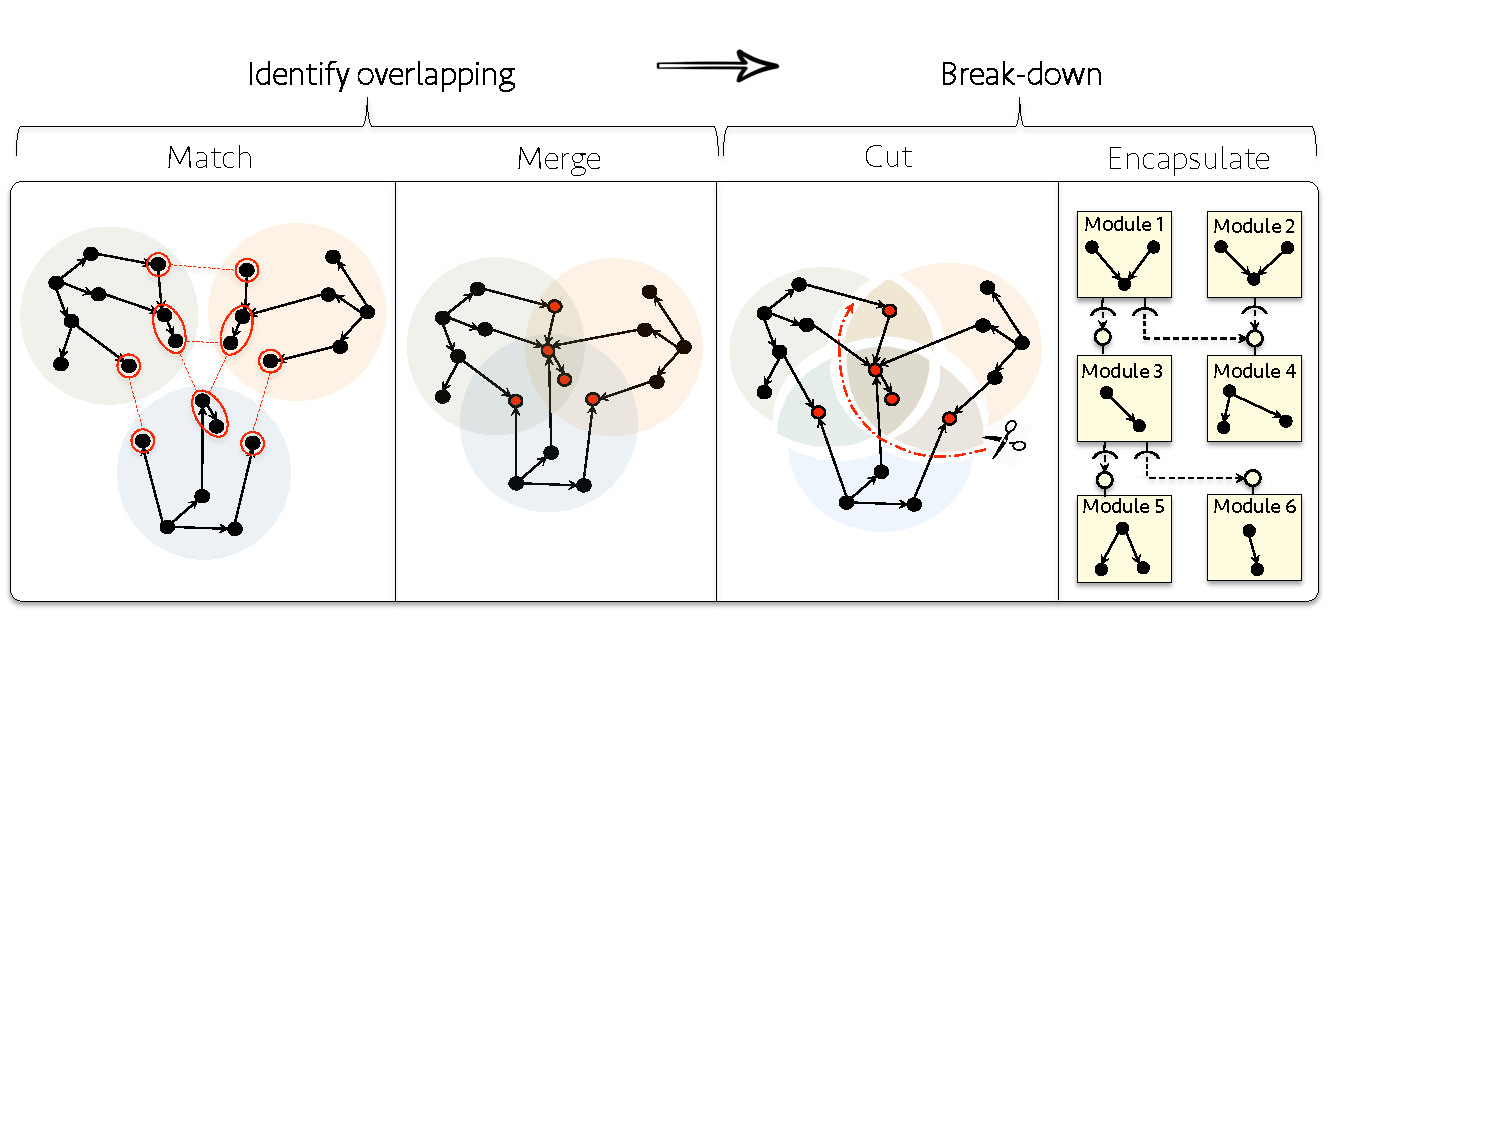
\includegraphics[width=1\linewidth]{images/breakdown.pdf}
\caption{Breaking down the input set by cutting overlapping}
\label{fig:breakingdown}
\end{figure}

\subsection{Identifying overlapping: \textit{match} and \textit{merge}}
\label{sec:identifyingoverlapping}

Our strategy to identify syntactic overlapping is based on the fact that a metamodel can be viewed as a directed graph $G=<V,A>$ where the vertexes $V$ represent metaclasses and the arcs $A$ represent references between metaclasses. Each DSL of the input set has a metamodel that represents its syntax. Syntactic overlapping is detected by identifying replicated vertex among all those graphs. Then, we organize the merged graphs in the form of a Venn diagram as illustrated in the two first steps shown in Figure \ref{fig:breakingdown}.

More concretely, our algorithm to identify syntactic overlapping is twofold. First, we perform a matching process that receives a set of graphs (one for each metamodel) and returns the collection of vertexes referencing metaclasses that are \textit{identical}. Second, we merge the matched vertexes, thus removing replications. In order to create the intersections, we store the information about what are the DSLs where the corresponding metaclass is defined.

Once matched vertexes are merged, we analyze the domain-specific actions associated to the corresponding metaclasses. Particularly, for each set of identical metaclasses we check if the domain-specific actions are equal as well. If so, they can considered as replicated code and we have semantic overlapping. Those domain-specific actions are merged.

In the case in which not all the domain-specific actions associated to two matched metaclasses are the same, we create different clusters of domain-specific actions, thus establishing a semantic variation point.

%\begin{equation}
%  Venn_{syn} : set(MM) \rightarrow set(<set(MM),set(MC)>)
%\end{equation}

%\begin{equation}
%  Venn_{syn}(mms) = \{<x,y> \mid x \in \mathcal{P}(mms), y = I_{syn}(x)\}
%\end{equation}

%Note that our algorithm relies on a function $I_{syn}$ that computes the intersection existing withing a given set of metamodels. It can be formalized as follows:

%\begin{equation}
%  I_{syn} : set(MM) \rightarrow set(MC)
%\end{equation}
%\vspace{-2mm}
%\begin{equation}
%  I_{syn}(mms) = \bigcap _{i=0}^{|mms|}mms_i
%\end{equation}

%Similarly, our algorithm for detecting \textbf{semantic intersections} can be described as a function that receives a set of aspects (one for each DSL of the input set) and returns a set of tuples containing all the intersections among these aspects. 

%\begin{equation}
%  Venn_{sem} : set(A) \rightarrow set(<set(A),set(DSA)>)
%\end{equation}

%\begin{equation}
%  Venn_{syn}(mms) = \{<x,y> \mid x \in \mathcal{P}(mms), y = I_{sem}(x)\}
%\end{equation}
%\vspace{2mm}

%This time, the algorithm for semantic commonalities relies on a function $I_{sem}$ that computes the intersection existing withing a given set of aspects. It can be formalized as follows:

%\begin{equation}
%  I_{sem} : set(A) \rightarrow set(DSA)
%\end{equation}
%\vspace{-2mm}
%\begin{equation}
%  I_{sem}(dsas) = \bigcap _{i=0}^{|dsas|}dsas_i
%\end{equation}

It is worth noting that detection of both syntactic and semantic overlapping relies on comparison of metaclasses and domain-specific actions respectively. At this point we need to clearly define such notion of equality that, as a matter of fact, is quite important to avoid alterations on the DSLs after the extraction of reusable language modules.

\vspace{-3mm}
\subsubsection{Comparison of metaclasses:} An operator for metaclasses comparison can be specified as follows: 

\begin{equation}
  \doteq~: MC \times MC \rightarrow bool
\end{equation}

To implement such operator, one can intuitively consider as a first approach the comparison of metaclasses names matching; two metaclasses are considered equal if their names are equal. Certainly, this approach results quite useful and it is quite probable that, we can find potential reuse. For example, one can expect that in a set of DSLs for finite state machines DSL, the construct \texttt{Transition} can be considered as a commonality.

Unfortunately, comparison of metaclasses by using only their names might have some problems. There are cases in which two metaclasses with the same name are not exactly the same because they do not represent the same domain concept, or because there are domains that use similar vocabulary. For instance, whereas in many cases the transitions of a state machine are only specified in terms of triggers and constraints, there are certain DSLs for state machines that allow to annotate transitions are annotated with time flags \cite{Graf:2007}.

In such cases, feasibility of potential reuse is not clear because the involved metaclasses offer different functionalities. Hence, a more restrictive operator should be considered. An approach that certainly helps is to compare metaclasses not only by their names but also by their attributes and references. Although this strategy can be quite restrictive, it guarantees that the detected reuse opportunities correspond to exact code clones so they can be extracted as reusable modules without any risk of altering the behavior of the DSLs.

In our approach we use the later strategy. Nevertheless, we consider that certain flexibility might be to define those operators. We provide an extensible approach where other operators (such as the surveyed in \cite{Lafi:2011}) can be easily incorporated.

%\vspace{-1mm}
%\begin{equation}
%\begin{split}
%  MC_{A} \doteq MC_{B} &= true \implies \\
%   & MC_{A}.name = MC_{B}.name
% \end{split}
%\end{equation}

%\begin{equation}
%  \doteqdot~: MC \times MC \rightarrow bool
%\end{equation}
%\vspace{-1mm}
%\begin{equation}
%\begin{split}
%  MC_{A} \doteqdot MC_{B} &= true \implies \\
%   & MC_{A}.name = MC_{B}.name ~ \wedge \\
%   & \forall a_1 \in MC_{A}.attr \mid (\exists a_2 \in MC_{B}.attr \mid a_1 = a_2) ~ \wedge \\
%   & \forall r_1 \in MC_{A}.refs \mid (\exists r_2 \in MC_{B}.refs \mid r_1 = r_2)
%  \end{split}
%\end{equation}

\vspace{-3mm}
\subsubsection{Comparison of domain-specific actions:} In turn, the operator for comparison of domain-specific actions can be specified as follows:

\begin{equation}
  \circeq~: DSA \times DSA \rightarrow bool
\end{equation}

Like methods in Java,domain specific actions have a signature that specifies its contract (i.e., return type, visibility, parameters, name, and so on), and a body where the behavior is actually implemented. In that sense, the implementation of a comparison operator for domain-specific actions can be performed by checking if their signatures are equal. This approach is practical and also reflects potential reuse; one might think that the probability that two domain-specific actions with the same signatures are the same is elevated.

However, during the conduction of this research we realized that there are cases in which signatures comparison is not enough. Two domain-specific actions defined in different DSLs can perform different computations even if they have the same signatures. For example, we can found semantic variation points in the implementation of DSLs for state machines where the domain-specific actions are implemented differently although their signatures are the same. As a result, we only guarantee potential reuse where we compare also the bodies of the domain-specific actions. 

Note that such comparison can be arbitrary difficult. Indeed, if we try to compare  the behavior of the domain-specific actions we will have to deal with the semantic equivalence problem that, indeed, is known to be undecidable \cite{Lucanu:2013}. To deal with this issue, we compare the body of domain-specific actions by in terms of its abstract syntax tree as proposed by Biegel et al \cite{Biegel:2010}. This strategy guarantees that semantic overlapping correspond to exact clones. Again, our approach can be extended to support other comparison operators for domain-specific actions. 

%\vspace{-1mm}
%\begin{equation}
%\begin{split}
%  DSA_{A} & \circeq DSA_{B} = true \implies \\
%   & DSA_{A}.name = DSA_{B}.name ~ \wedge \\
%   & DSA_{A}.returnType = DSA_{B}.returnType ~ \wedge \\
%   & DSA_{A}.visibility = DSA_{B}.visibility ~ \wedge \\
%   & \forall p_1 \in DSA_{A}.params \mid (\exists p_2 \in %DSA_{B}.params \mid p_1 = p_2)
% \end{split}
%\end{equation}

%\begin{equation}
%  \triangleq~: DSA \times DSA \rightarrow bool
%\end{equation}
%\vspace{-1mm}
%\begin{equation}
%\begin{split}
%  DSA_{A} & \circeq DSA_{B} = true \implies \\
%   & DSA_{A}.name = DSA_{B}.name ~ \wedge \\
%   & DSA_{A}.returnType = DSA_{B}.returnType ~ \wedge \\
%   & DSA_{A}.visibility = DSA_{B}.visibility ~ \wedge \\
%   & \forall p_1 \in DSA_{A}.params \mid (\exists p_2 \in DSA_{B}.params \mid p_1 = p_2)  ~ \wedge \\
%   & DSA_{A} \circeq DSA_{B} ~ \wedge \\
%   & DSA_{A}.AST = DSA_{B}.AST
% \end{split}
%\end{equation}


%It is worth nothing that there is this phenomenon of \textit{semantical variability}. A necessary condition to decide whether two language constructs are equivalent is that both, the metaclass and the associated domain-specific actions are equivalent. This condition guarantees that the specification is the same not only at the level of the abstract syntax but also at the level of the semantics. However, there is a phenomenon in the literature that corresponds to semantical variability \cite{Cengarle:2009}. There is semantical variability when there there are two constructs that have the same abstract syntax (i.e., their metaclasses are equal) but that differ in the domain-specific actions. This case is of interest for us because even in the presence of semantical variability we can have some potential reuse. If the metaclasses of two constructs are the same we can reuse them even if their domain-specific actions are different. 

%\vspace{-2mm}
%\subsubsection{Visualizing semantical variability:} Note that the phenomenon of semantical variability is evident in the example presented. Where there are syntactic commonalities between DSLs Logo and FSM, there are not semantic commonalities. As an additional feature of our approach, we provide a visualization of the semantical variability phenomenon. The idea is that language designers can see what are the variations in the domain specific actions.
%\todo[inline]{Usa el ejemplo para ejemplificar}

\subsection{Breaking down the input set: \textit{cut} and \textit{encapsulate}}

After being identified overlapping among the DSLs in the input set, we extract a set of reusable language modules. To this end, we adopt the idea presented by V\"oelter et al \cite[p. 60-61]{voelter:2013}: we break-down the overlapping by creating one language module for each different intersection as illustrated in the third step of Figure \ref{fig:breakingdown}. The reasoning to this solution is quite simple: by definition, an intersection is a set of language constructs that are shared by two or more DSLs. If we extract those language constructs in separated language modules, the language module can be defined once and reused by all the DSLs that require it. So, we can consider that the extracted language module is reusable. 

In our approach, we implemented this separation of overlapping as a graph partitioning algorithm. The algorithm receives the graph(s) obtained from the merging process and returns a set of vertex clusters: one cluster for each intersection of the Venn diagram. Arcs defined between vertexes in different clusters can be considered as cross-cutting dependencies between clusters. Then, we encapsulate each vertex cluster in the form of language modules. Each module contains a metamodel, a set of domain-specific actions, and a set of dependences towards other language modules. 

Dependencies between language modules are supported by means of the classical required and provided roles in components-based software development. There is a \textit{requiring module} that uses some constructs provided by a \textit{providing module}. The requiring module has a dependency relationship towards the providing one that, in the small, is materialized by the fact that some of the classes of the requiring module have references (simple references, containment references, or inheritances) to some constructs of the providing one. In order to avoid direct references between modules, we introduce the notion of interfaces for dealing with modules' dependencies. The requiring language has a \textit{required interface} whereas the providing one has the \textit{provided interface}. A required interface contains the set of constructs required by the requiring module which are supposed to be replaced by actual construct provided by other module(s) (see Figure \ref{fig:approaches-interfaces}).

We use \textit{model types} \cite{Steel:2007} to express both required and provided interfaces. A module can have some references to the constructs declared in its required interface. In turn, the relationship between a module and its provided interface is \textit{implements} (deeply explained in \cite{Degueule:2015}). A module implements the functionality exposed in its model type. If the required interface is a subtype of the provided interface, then the provided interface fulfills the requirements declared in a required interface. 

\begin{figure}
\centering
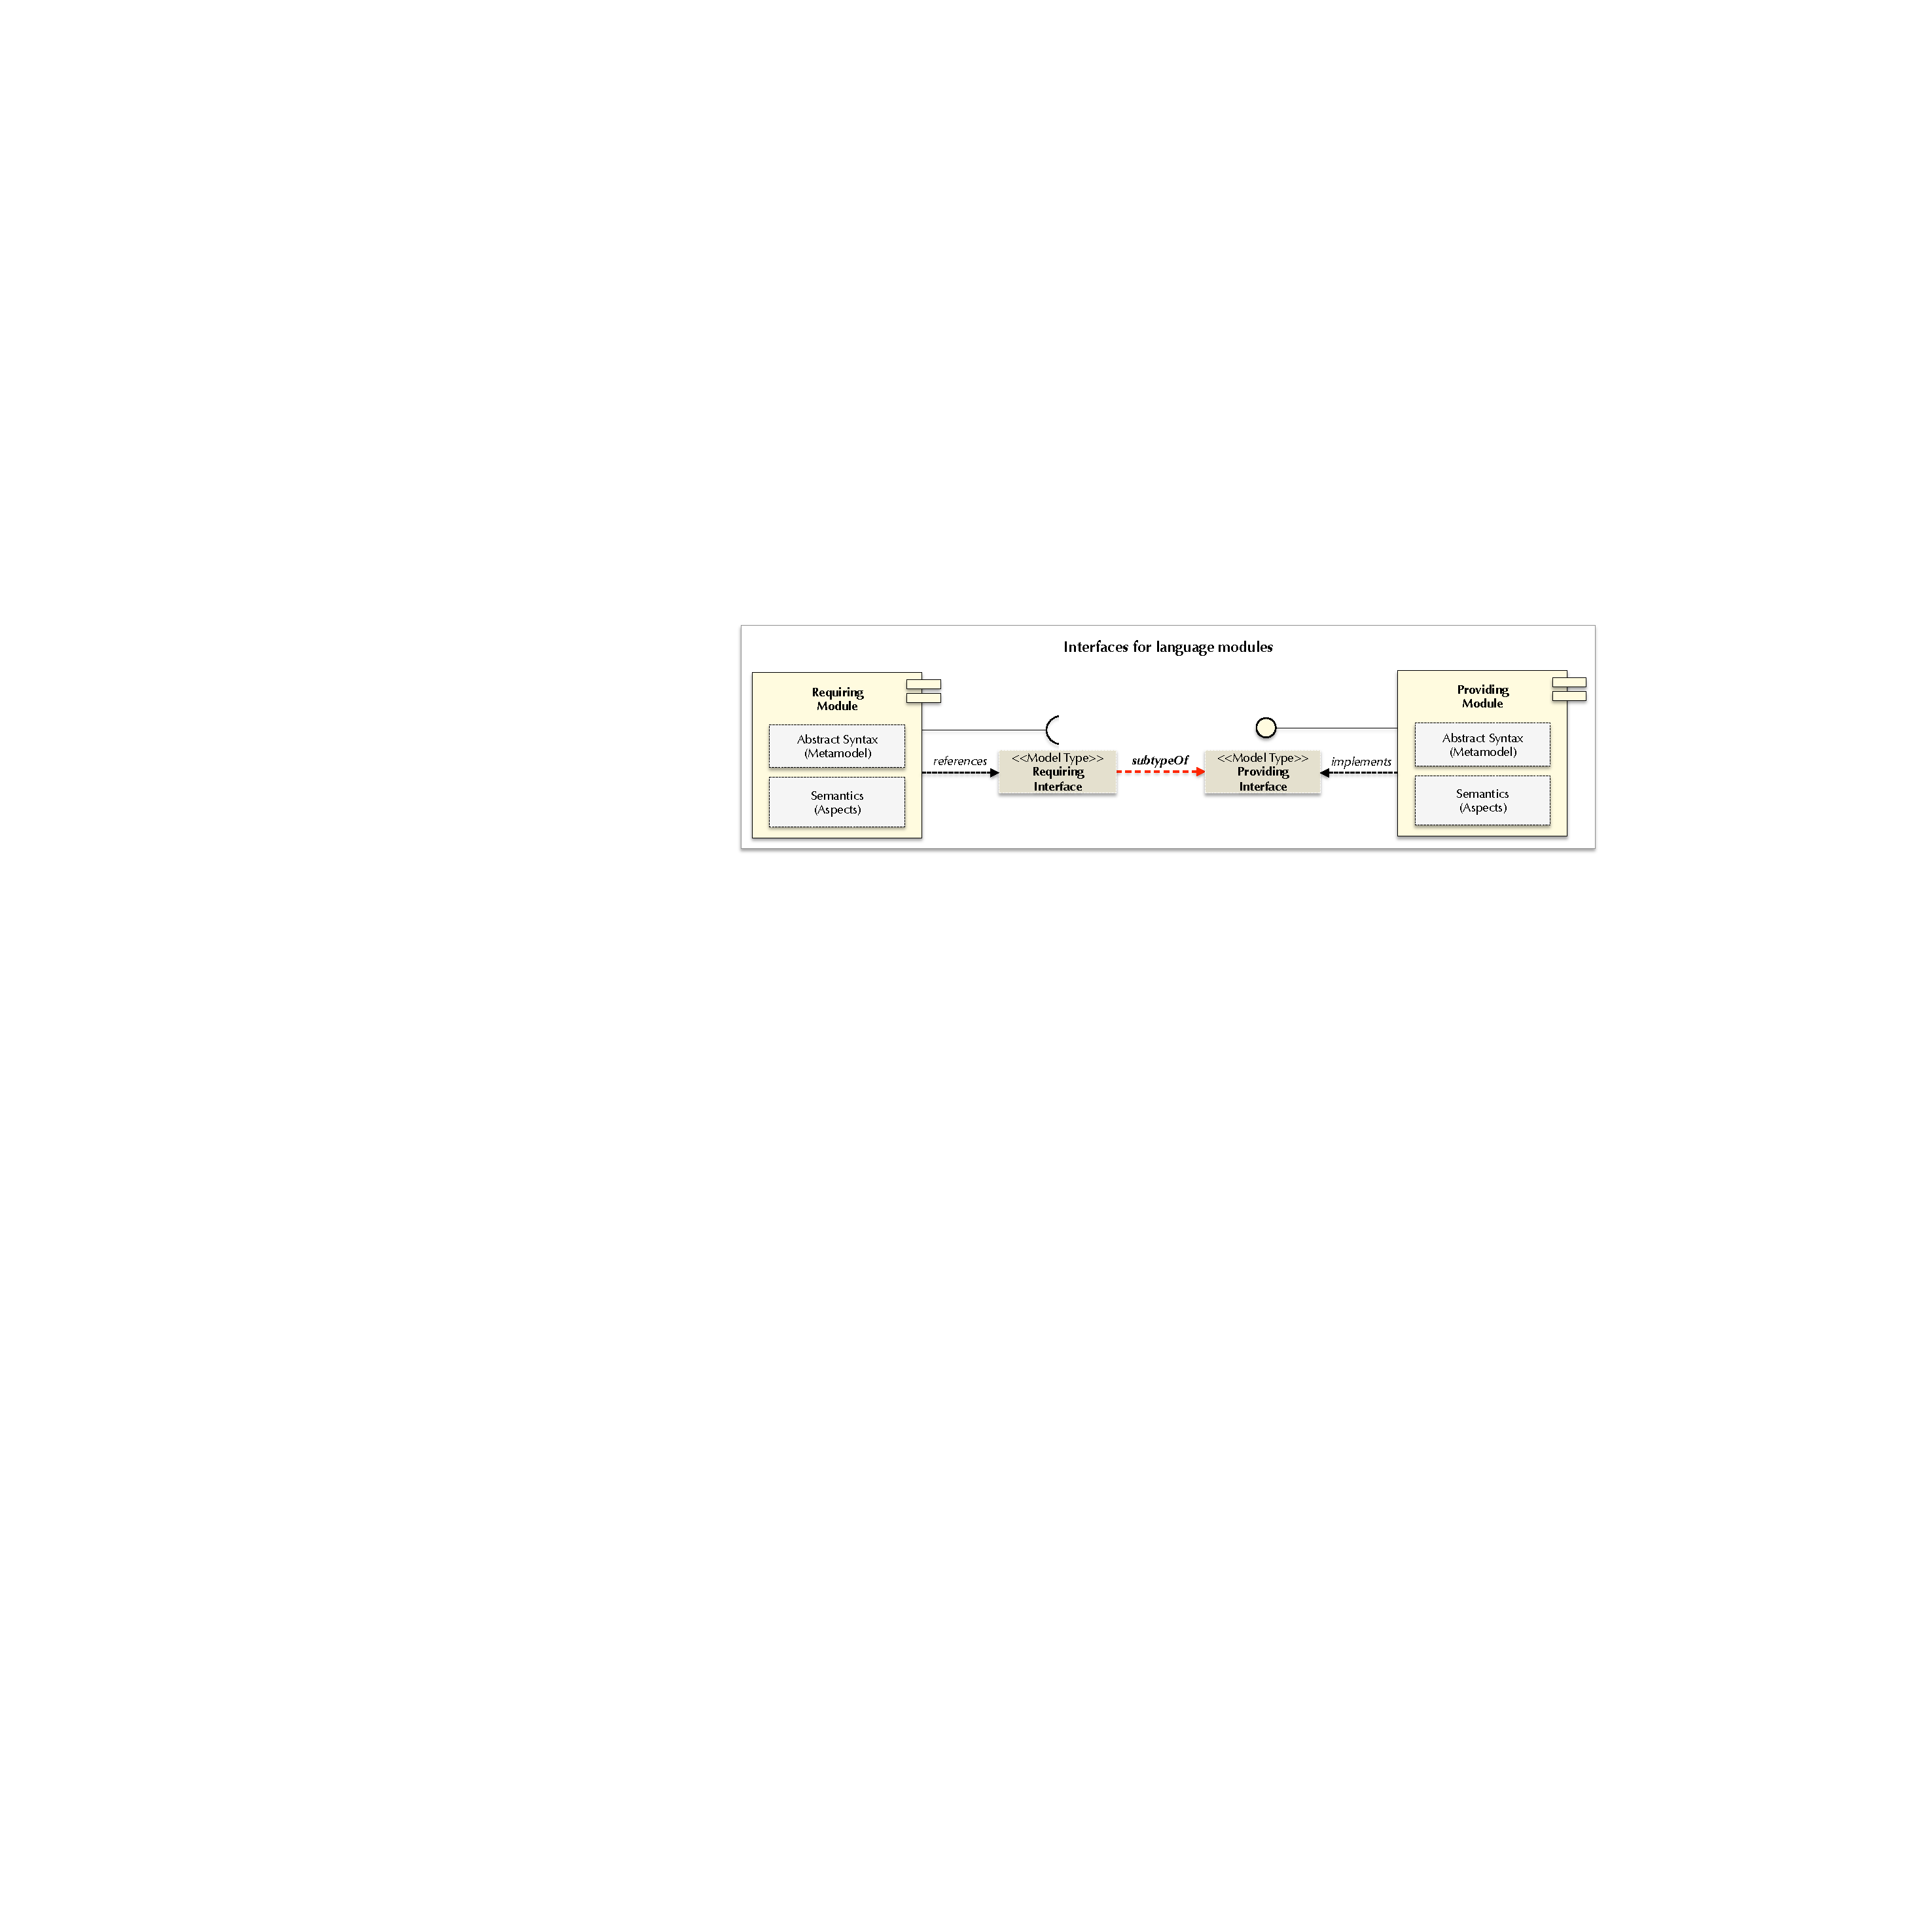
\includegraphics[width=1\linewidth]{images/approach-interfaces.pdf}
\caption{Interfaces for language modules}
\label{fig:approaches-interfaces}
\end{figure}
\vspace{-3mm}
